\documentclass{article}

\usepackage{graphicx} % Used for adding images
\usepackage{wrapfig} % Used for wrapping figures inside text
\usepackage{blindtext} % Used for putting dummy text

\title{Adding Images in Latex}
\author{Irfan}
\date{\today}
% Defines the folder where images are located. Note the dual curly braces
\graphicspath{{./}}

\begin{document}

\maketitle

\listoffigures % This will list all figures in the document
\listoftables % This will list all tables in the document

\section{Adding and scaling image}
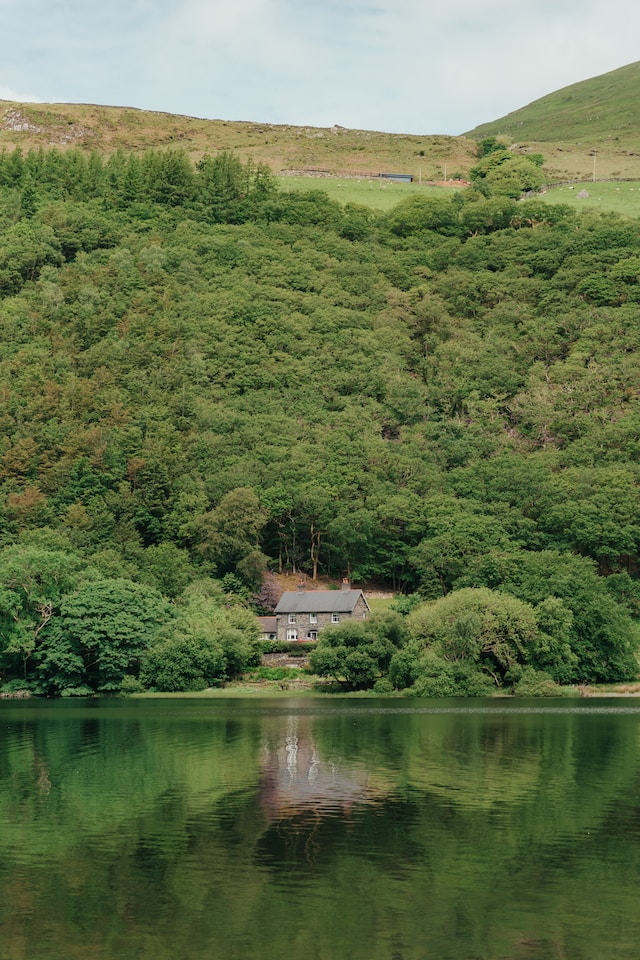
\includegraphics[scale=0.2]{shawnanggg-SQ9Q1nvwhlI-unsplash.jpg}

\section{Setting width and height manually}

\subsection{Using centimeters as unit}
  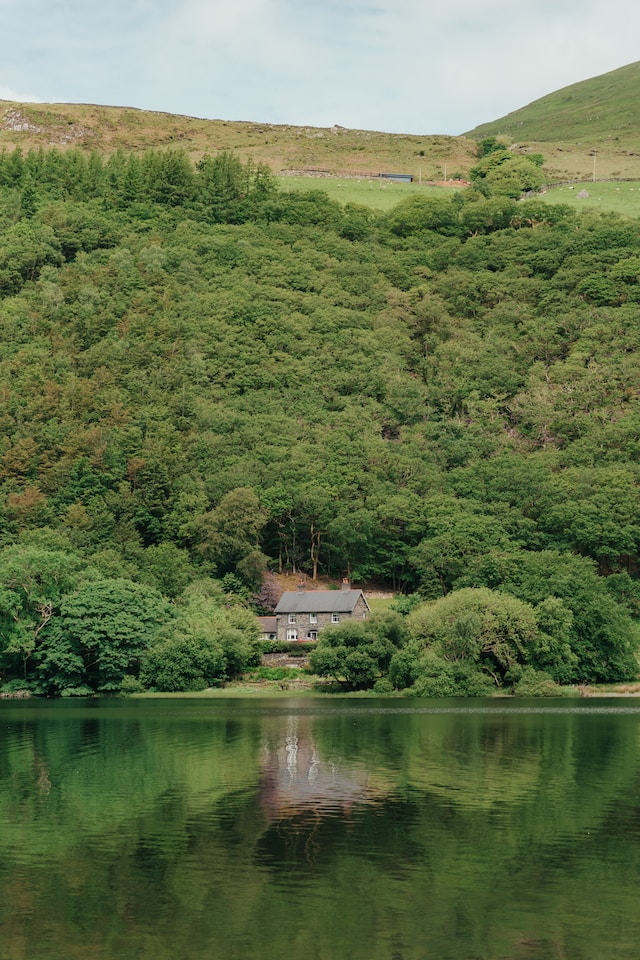
\includegraphics[width=5cm, height=10cm]{shawnanggg-SQ9Q1nvwhlI-unsplash.jpg}

\subsection{Using inches as unit}
  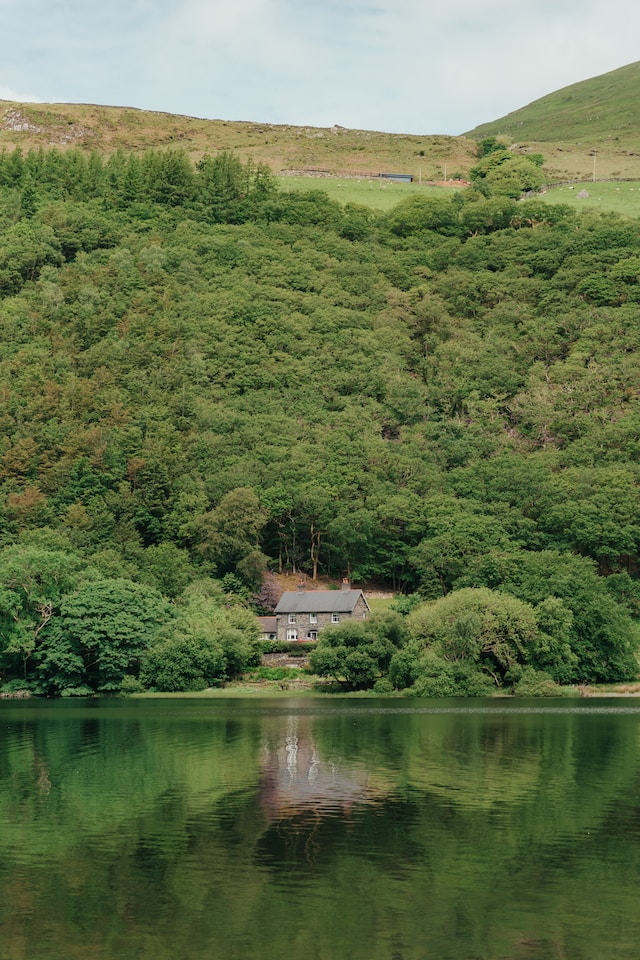
\includegraphics[width=2in]{shawnanggg-SQ9Q1nvwhlI-unsplash.jpg}

\subsection{Using textwidth as unit}
  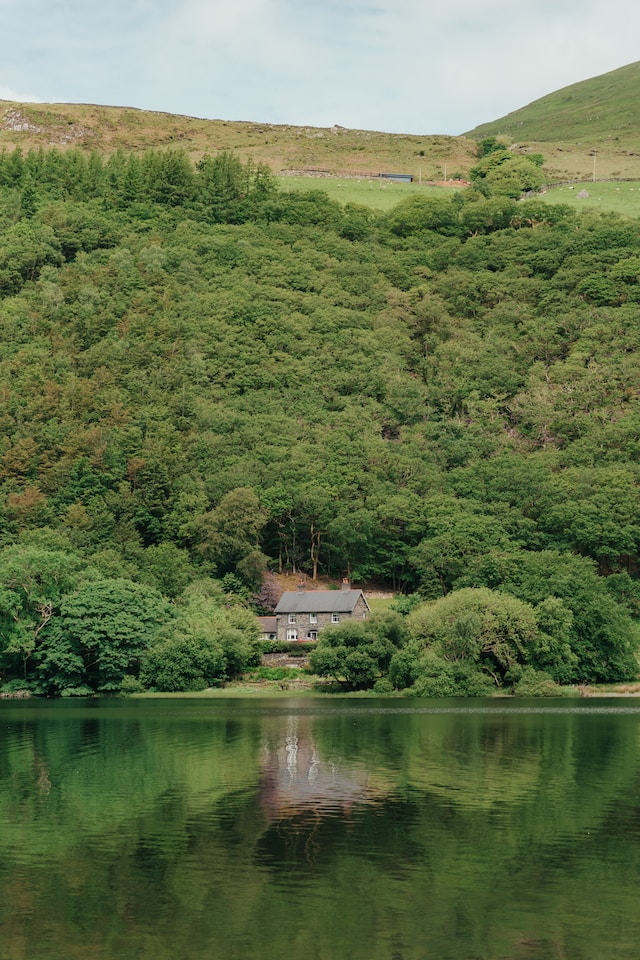
\includegraphics[width=0.5\textwidth]{shawnanggg-SQ9Q1nvwhlI-unsplash.jpg}

\section{The figure environment}
% In Latex, images are inline by default. If we want to avoid this, we can
% wrap images in the "figure" environment.
\begin{figure}[h]
\caption{An Example Image}
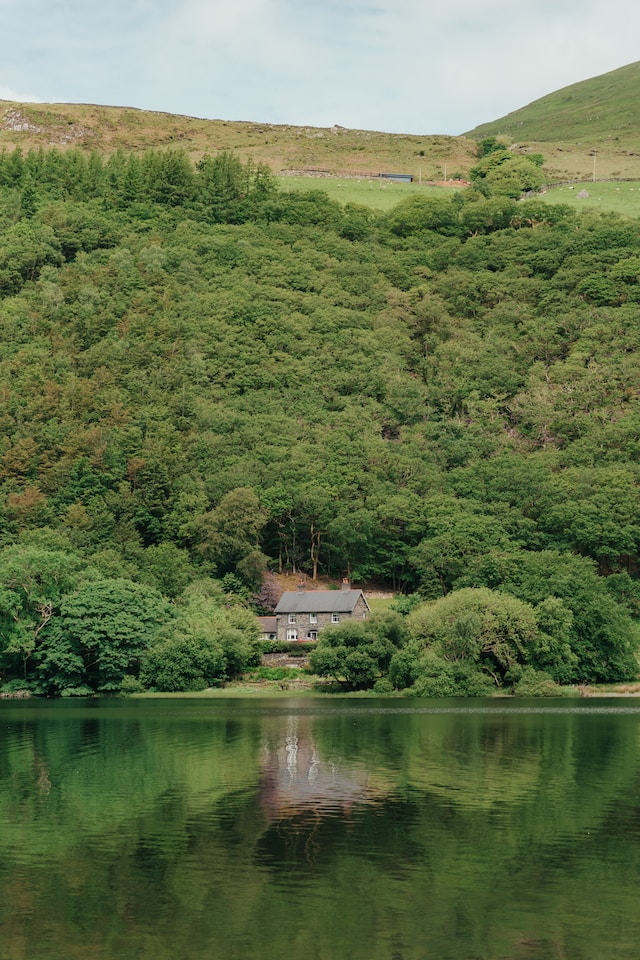
\includegraphics[width=0.5\textwidth]{shawnanggg-SQ9Q1nvwhlI-unsplash.jpg}
\end{figure}

\newpage

\subsection{Centered figure}
  \begin{figure}[h!]
  \caption{A Centered Image}
  \centering
  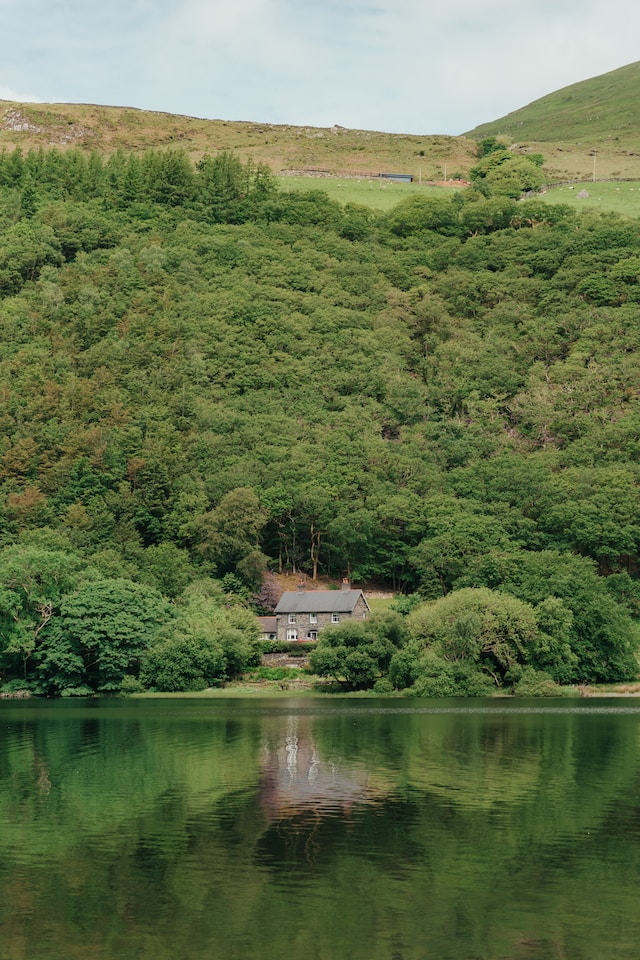
\includegraphics[width=3cm]{shawnanggg-SQ9Q1nvwhlI-unsplash.jpg}
  \end{figure}

\subsection{Left aligned figure}
  \begin{figure}[h!]
  \caption{A Right Aligned Image}
  \raggedleft
  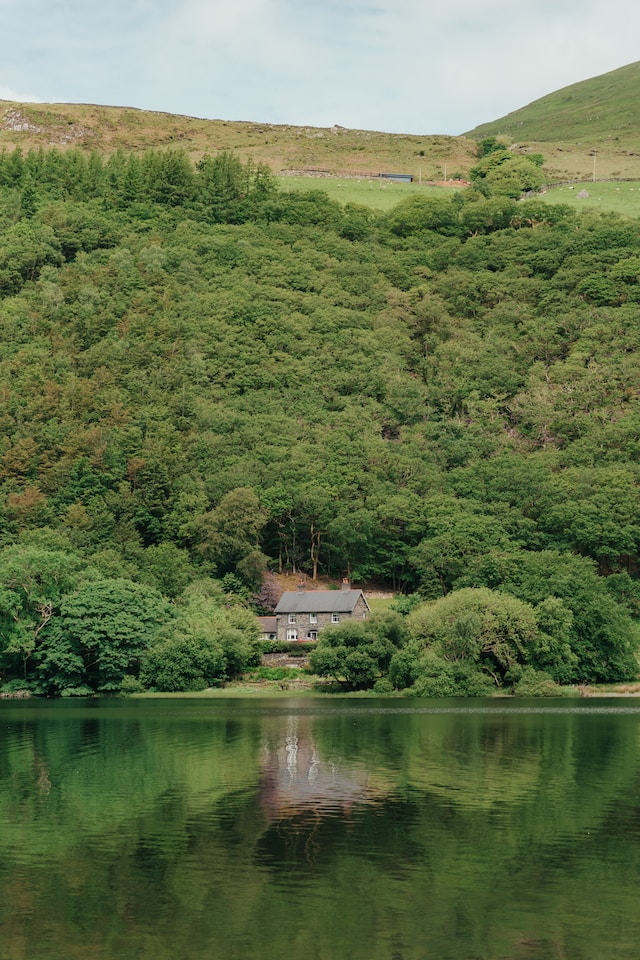
\includegraphics[width=3cm]{shawnanggg-SQ9Q1nvwhlI-unsplash.jpg}
  \end{figure}

\newpage

\section{Wrapping figures inside text}
% To wrap figures inside text, use the "wrapfigure" environment
% 'l' means left align. We also have to pass the width of image in the options
\begin{wrapfigure}{l}{3cm}
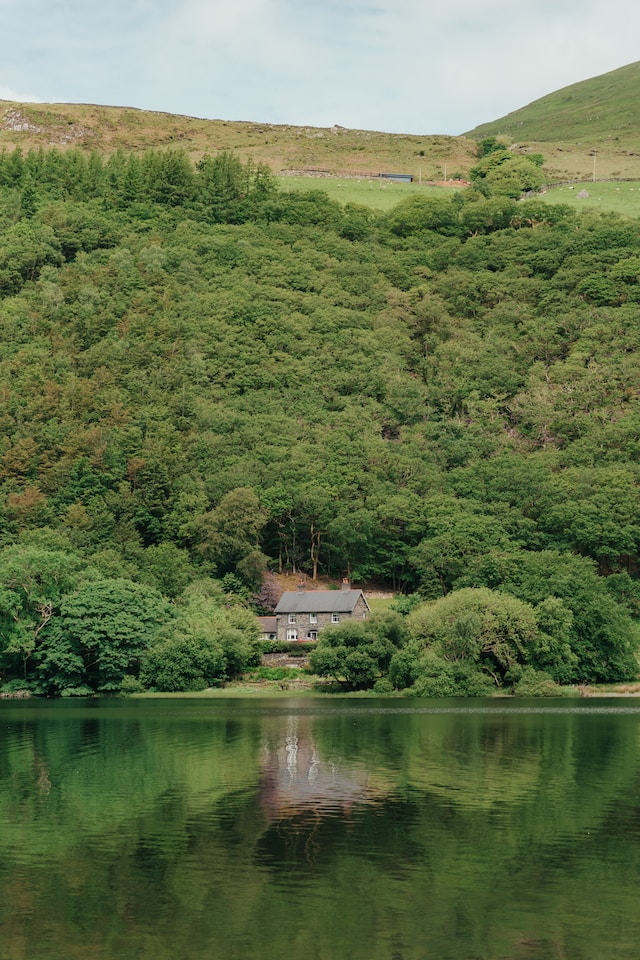
\includegraphics[width=3cm]{shawnanggg-SQ9Q1nvwhlI-unsplash.jpg}
\caption{Wrapped Image}
\end{wrapfigure}

\blindtext
\end{document}
